\documentclass[12pt]{article}

\usepackage{listings}
\usepackage{color}

\definecolor{dkgreen}{rgb}{0,0.6,0}
\definecolor{gray}{rgb}{0.5,0.5,0.5}
\definecolor{mauve}{rgb}{0.58,0,0.82}

\lstset{frame=tb,
  language=C++,
  aboveskip=3mm,
  belowskip=3mm,
  showstringspaces=false,
  columns=flexible,
  basicstyle={\small\ttfamily},
  numbers=none,
  numberstyle=\tiny\color{gray},
  keywordstyle=\color{blue},
  commentstyle=\color{dkgreen},
  stringstyle=\color{mauve},
  breaklines=true,
  breakatwhitespace=true,
  tabsize=3
}

\usepackage{color}
\usepackage{float}
\usepackage{answers}
\usepackage{setspace}
\usepackage{graphicx}
\usepackage{enumitem}
\usepackage{multicol}
\usepackage{mathrsfs}
\usepackage[margin=1in]{geometry} 
\usepackage{amsmath,amsthm,amssymb}
 
\newcommand{\N}{\mathbb{N}}
\newcommand{\Z}{\mathbb{Z}}
\newcommand{\C}{\mathbb{C}}
\newcommand{\R}{\mathbb{R}}

\DeclareMathOperator{\sech}{sech}
\DeclareMathOperator{\csch}{csch}
 
\newenvironment{theorem}[2][Theorem]{\begin{trivlist}
\item[\hskip \labelsep {\bfseries #1}\hskip \labelsep {\bfseries #2.}]}{\end{trivlist}}
\newenvironment{definition}[2][Definition]{\begin{trivlist}
\item[\hskip \labelsep {\bfseries #1}\hskip \labelsep {\bfseries #2.}]}{\end{trivlist}}
\newenvironment{proposition}[2][Proposition]{\begin{trivlist}
\item[\hskip \labelsep {\bfseries #1}\hskip \labelsep {\bfseries #2.}]}{\end{trivlist}}
\newenvironment{lemma}[2][Lemma]{\begin{trivlist}
\item[\hskip \labelsep {\bfseries #1}\hskip \labelsep {\bfseries #2.}]}{\end{trivlist}}
\newenvironment{exercise}[2][Exercise]{\begin{trivlist}
\item[\hskip \labelsep {\bfseries #1}\hskip \labelsep {\bfseries #2.}]}{\end{trivlist}}
\newenvironment{solution}[2][Solution]{\begin{trivlist}
\item[\hskip \labelsep {\bfseries #1}]}{\end{trivlist}}
\newenvironment{problem}[2][Problem]{\begin{trivlist}
\item[\hskip \labelsep {\bfseries #1}\hskip \labelsep {\bfseries #2.}]}{\end{trivlist}}
\newenvironment{question}[2][Question]{\begin{trivlist}
\item[\hskip \labelsep {\bfseries #1}\hskip \labelsep {\bfseries #2.}]}{\end{trivlist}}
\newenvironment{corollary}[2][Corollary]{\begin{trivlist}
\item[\hskip \labelsep {\bfseries #1}\hskip \labelsep {\bfseries #2.}]}{\end{trivlist}}
 
\begin{document}
% --------------------------------------------------------------
%                         Start here
% --------------------------------------------------------------
 
\title{\textbf{HW9}}%replace with the appropriate homework number
\author{Seyed Armin Vakil Ghahani\\ %replace with your name
PSU ID: 914017982\\
CSE-565 Fall 2018\\
Collaboration with:
Sara Mahdizadeh Shahri, Soheil Khadirsharbiyani,\\
Muhammad Talha Imran} %if necessary, replace with your course title}
 
\maketitle
%Below is an example of the problem environment
\begin{problem}{1}
Flow and cut example
\end{problem}

%Below is the solution environment
\begin{solution}{}
\begin{itemize}
\item a) The value of this flow is $5+8+5 = 18$. This flow is not maximum 
because there is an augmenting path in the residual graph: $s, u, v, w, d, t$.
After adding this augmenting path to the graph and updating flow, we have a
flow of $5+8+8=21$. Moreover, after this there will not be any augmenting
path, and consequently, the maximum flow is 21.
\item b) The minimum s-t cut is $(A=\{s, u, v, w\}, V-A)$, and its capacity is
the sum of these edges: $\{(s,d), (w,d), (u,t), (v,t)\}$ that is $5+3+8+5=21$. All of the outcoming edges from this set have the maximum
flow that they can have. Moreover, all of the incoming edges to this set
have zero flow.
\end{itemize}
\begin{figure}[H]
 \centering
 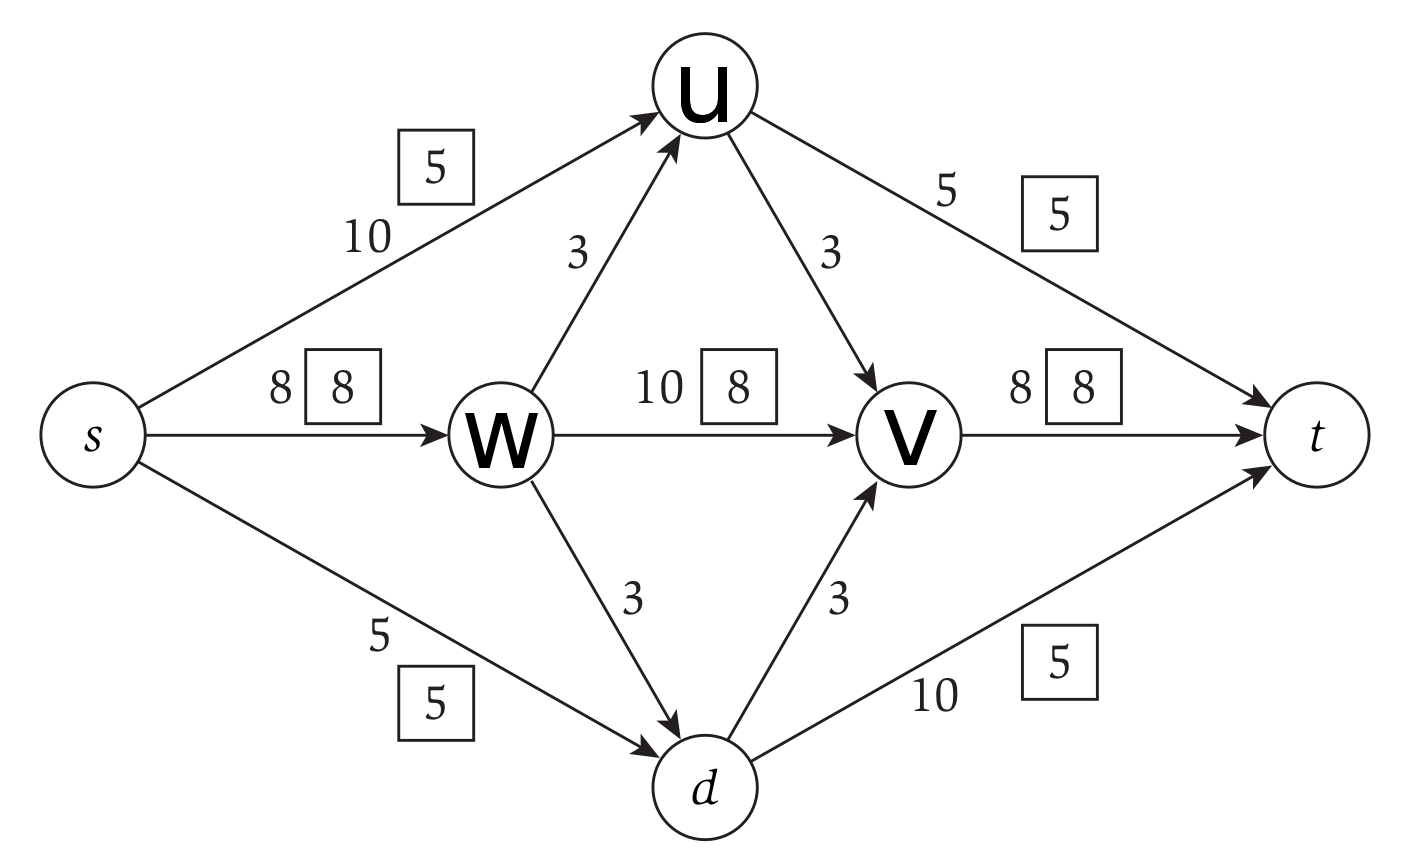
\includegraphics[width=0.80\textwidth]{q1.png}
 \caption{
 \label{fig:1a}}
\end{figure}
\end{solution}


\begin{problem}{2}
How bad is a greedy flow?
\end{problem}

%Below is the solution environment
\begin{solution}{}
This statement is wrong because we can create a graph that its maximum flow
is $b$, however, this greedy algorithm may result 1. As a result, there is 
not any constant which the given statement becomes true.

Suppose a graph that have $2*b+2$ vertices as it shown below. If the greedy 
algorithm chooses the path with bold edges, and remove the forwarding edges
from the graph, there will not be any path from s to t. As a result, this 
fast algorithm returns a flow of 1.
\begin{figure}[H]
 \centering
 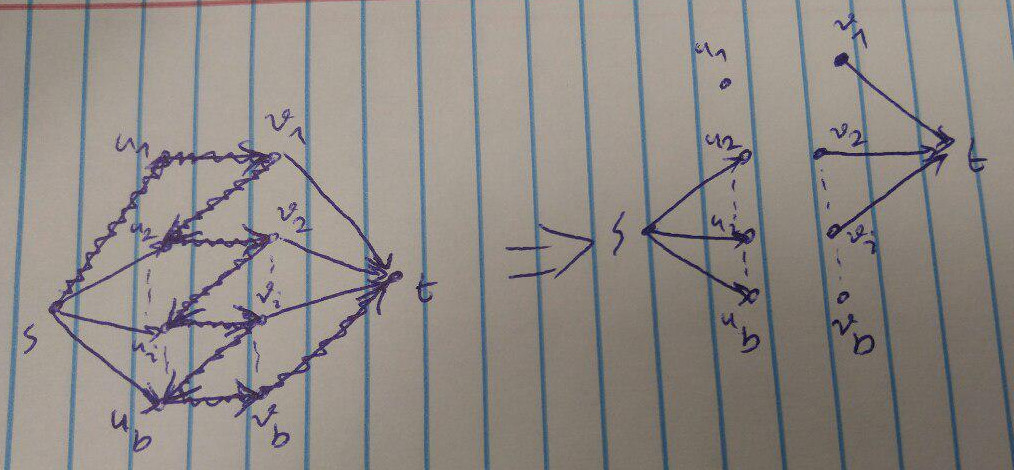
\includegraphics[width=0.80\textwidth]{q2.jpg}
 \caption{Problem 2 sample
 \label{fig:2a}}
\end{figure}
\end{solution}


\begin{problem}{3}
Algorithm to delete k edges
\end{problem}

%Below is the solution environment
\begin{solution}{}
Suppose that we run the maximum flow algorithm in this graph and we have 
calculated the minimum (s-t) cut in this graph. If the capacity of this 
minimum cut is less than or equal to $k$, we can easily remove the edges
in this cut, and consequently, in the remaining graph there is not any
path from s to t, and the flow will be zero (the smallest possible value).

On the other hand, if this minimum cut have more than $k$ edges (Suppose
that the minimum cut is $f$), we can randomly choose $k$ edges from this
cut and the maximum flow of remaining graph will be at most $f-k$. Its 
because in the new graph $G^\prime$, the capacity of every s-t cut is
reduced at most $k$. As a result, since the minimum s-t cut was $f$ before,
the minimum s-t cut in $G^\prime$ is at least $f-k$. Thus, the maximum
flow in $G^\prime$ is at most $f-k$.
\end{solution}


\begin{problem}{4}
Product of Polynomials
\end{problem}

%Below is the solution environment
\begin{solution}{}
\begin{itemize}
\item a) The asymptotic running time of multiplying two polynomial of degree
n and m, respectively, is $O(nm)$. As a result, the running time of first
multiplication is $O(n^2)$, and the result will be a polynomial of degree
$2*n-1$.

In the next step, the running time of the second multiplication is 
$O(2*n*n)$, and the result will be a polynomial of degree $3*n-1$.

In the $i^{th}$ step, the running time of the $i^{th}$ multiplication is
$O(i*n*n)$, and the result will be a polynomial of degree $(i+1)*n-1$.

Actually, the recurrence equation of calculating $P_0*P_1 * ... * P_{i-1}$
is $T(i) = T(i-1) + O(i*n*n)$. As a result, the running time of this 
algorithm will be $\sum_{i=1}^{n-1} c*i*n^2 = c*n^2*\sum_{i=1}^{n-1} i = 
c * n^2 * n * (n-1) / 2 = O(n^4)$.

\item b) We can calculate the result of the first $n/2$ multiplications,
and the second $n/2$ multiplications separately, and after that multiplying
the two polynomials with degree of $(n/2)*n-1$. Hence, the recurrence 
equation of calculating the result in this way is $T(n) = 2T(n/2) + O(n^4/4)$. Hence, the running time of this algorithm based on the Master
Theorem is $O(n^4)$. The asymptotic running time of this part and the 
previous are equal, however, the constant time of the algorithm of this 
part is significantly lower.

\item c) We know that multiplying two polynomial with degree of $n$ is
$O(nlogn)$. As a result, the recurrence equation of part b changes to this:
$T(n) = 2T(n/2) + O((n/2*n-1) * log(n/2*n-1))$ or $T(2^k) = 2T(2^{k-1}) +
O(\frac{2^k*2^k}{2} * log(\frac{2^k*2^k}{2}))$. Hence, $T(2^k) = 2T(2^{k-1})
+ O(2^{2k-1} * (2k-1))$. In this equation, we can change $2^k$ to $p$, and
consequently, we have this equation: $T(p) = 2T(p/2) +
O(\frac{p^2}{2}*log(p))$. As a result, by the Master Theorem, $T(p) \in 
O(p^2*log^2(p))$, and if we change $p$ to $2^k$ and $n$, we have
this: $T(n) \in O(n^2 * log^2(n))$.
\item d, e) I want to go for a 30\% option.
\end{itemize}
\end{solution}


\pagebreak

\end{document}

